%\documentclass[oldversion,referee]{aa}
\documentclass[]{aa}
%\documentclass[]{aa}
\usepackage{graphicx}
\usepackage{psfig}
\usepackage{epstopdf}
\usepackage{amssymb}
\usepackage{amsmath}
\usepackage{verbatim}
\usepackage{natbib}
\usepackage{rotate}
\usepackage{lscape}
%\usepackage{dsfont}
\usepackage{aalongtable}
\usepackage{supertabular}
\usepackage{mathbbol}
\usepackage{bm}
\usepackage{mathtools}
%\usepackage[subnum]{cases}
\usepackage{enumerate}
\usepackage{draftcopy}
\usepackage{algorithm}
\usepackage{algpseudocode}
\usepackage{pifont}

\usepackage{caption}
\usepackage{subcaption}
%\psdraft
%\usepackage{hyperref}
\usepackage{arydshln}
\usepackage{amsmath}
\bibpunct{(}{)}{;}{a}{}{,}

\newcommand{\tbsp}{\rule{0pt}{18pt}}
\newcommand\sqdeg{deg$^{2}$}
\newcommand\psqdeg{deg$^{-2}$}
\newcommand\ugriz{u$^*$g'r'i'z'}
\newcommand\mic{$\mu$m}
\newcommand\AAn{\AA~}
\newcommand\sfr{SFR$_{0.5}$}
\newcommand\ssfr{sSFR$_{0.5}$}
\newcommand\msol{\mbox{M$_{\odot}$}}
\newcommand\wph{W.Hz$^{-1}$}
\newcommand\lsol{\mbox{L$_{\odot}$}}
\newcommand{\appropto}{\mathrel{\vcenter{
  \offinterlineskip\halign{\hfil$##$\cr
    \propto\cr\noalign{\kern2pt}\sim\cr\noalign{\kern-2pt}}}}}
%\usepackage{newtxtext,newtxmath}



\def\mathY{\bm{\mathcal{Y}}}
%\def\mathY{\bm{\mathcal{V}}}
\def\Bchi{\large\bm{\mathcal{\chi}}}
%\def\Bchi{\chi}
\def\PVec{\textbf{x}}
%\input{Defs.tex}


 \def\supertiny{ \font\supertinyfont = cmr10 at 4pt \relax \supertinyfont}
 
 
\begin{document}      

	      
\title{Fast Scheme to Approximate an Offset Point Spread Function Response}

\subtitle{}
%\author{M. Atemkeng$^{1}$\thanks{E-mail: m.atemkeng@gmail.com}, O. Smirnov$^{12}$, 
% C. Tasse$^{13}$, G. Foster$^{12}$, J. Jonas$^{12}$}
\institute{
Department of Physics \& Electronics, Rhodes University, PO Box 94,
Grahamstown, 6140, South Africa
\and
SKA South Africa, 3rd Floor, The Park, Park Road, Pinelands, 7405, South Africa
\and
GEPI, Observatoire de Paris, CNRS, Universit\'e Paris Diderot,
5 place Jules Janssen, 92190 Meudon, France
}
%   \author{}
%   \offprints{}
%   \institute{}
\date{Received  / Accepted }


\abstract{
}

\authorrunning{N. Bourbaki}



%% \authorrunning{}
\titlerunning{Beyond PSF}
   \maketitle



\section{Introduction}
\section{Motivation}
\section{Matrix formulation of the problem - 1D interferometer}

Here I intend to use convolution matrices properties to {\it qualitatively} study how ``pseudo-PSF'' vary as a
function of source location. Here I limit myselves to a 1-dimensional
interferometer (scalar only), so that
Convolution matrices are Toeplitz-symetyric (see bellow). In a more
general case, (along my intuition - but should be thought more
carefully), convolution matrices should be block-Toeplitz (each
block is a Toeplitz), while symetricity should still be true. 

\subsection{Remarks on the convolution and linear algebra}

In functional form the convolution theorem can be written as follows:


\def\F{\mathcal{F}}
\def\Fm{\bm{F}}
\def\Gauss{\bm{\mathcal{G}}}
\def\conv{\mathcal{*}}

\begin{alignat}{2}
%\label{eq:Lin}
%\F \left{ a.b\right}=&\F \left{ a\right}.\F \left{b\right}\\
\F \left\{  a.b\right\}=& \F \left\{a\right\}\conv\F \left\{b\right\}
\end{alignat}

Noting the convolution product is linear, we can reexpress the
convolution product and associated theorem asing linear
transformations:

\newcommand{\C}[1]{\bm{\mathcal{C}}_{#1}}
\newcommand{\vv}[1]{\bm{#1}}
\def\one{\bm{1}}


\begin{alignat}{2}
\label{eq:ConvTh}
%\F \left{ a.b\right}=&\F \left{ a\right}.\F \left{b\right}\\
\Fm \vv{A}\vv{b}=& \C{\vv{A}}\Fm \vv{b}
\end{alignat}

\noindent where $\Fm$ is the Fourier operator of size 
$n_{uv}\times n_{lm}$ ($\Fm$ is unitary $\Fm^H\Fm=\one$), $\vv{b}$ is
a vector with size $n_{lm}$. The matrix $\vv{A}$ models the scalar
multiplication of each point in $\vv{b}$, and is therefore diagonal of
size $n_{lm}\times n_{lm}$, and $\C{\vv{A}}$ is the convolution matrix
of size $n_{uv}\times n_{uv}$. There is a bijective relation

\begin{alignat}{2}
\label{eq:ConvTh}
%\F \left{ a.b\right}=&\F \left{ a\right}.\F \left{b\right}\\
\vv{A} \longleftrightarrow \C{\vv{A}}
\end{alignat}
 
\noindent in the sense that a scalar multiplucation defines a convolution
function and conversely. The matrices $\vv{A}$ and $\C{\vv{A}}$ always
have the following properties:

\begin{itemize}
  \item $\vv{A}$ is diagonal

   \item In the 1D case
\begin{itemize}
  \item $\C{\vv{A}}$ is Toeplitz
  \item In addition, for radiointerferometry, because the uv plane is symetric, $\C{\vv{A}}$ is symetric
\end{itemize}

\end{itemize}

The matrix $\C{\vv{A}}$ being Toeplitz, each row $\left[ \C{\vv{A}}
  \right]_l$ with sky coordinate $l$ can be built using a
rolling operator $\Delta_l$ that shifts the first row (the PSF at the field
center for example) to location of row $l$:

\begin{alignat}{2}
\label{eq:ConvTh}
%\F \left{ a.b\right}=&\F \left{ a\right}.\F \left{b\right}\\
\left[ \C{\vv{A}} \right]_l =& \Delta_l \left\{ \left[ \C{\vv{A}} \right]_0 \right\}
and&\\
\left[ \C{\vv{A}} \right]_0 =& \Fm^H \ \text{diag}(\vv{A})
\end{alignat}

The rolling operator is essentially just a reindexing, and has the
following properties:

\begin{alignat}{2}
\label{eq:PropsDelta0}
%\F \left{ a.b\right}=&\F \left{ a\right}.\F \left{b\right}\\
\Delta_l \left\{ a\vv{x} \right\} =&  a \Delta_l \left\{\vv{x} \right\} \\
\label{eq:PropsDelta1}
\Delta_l \left\{ \sum_i \vv{x}_i \right\} =& \sum_i \Delta_l \left\{ \vv{x}_i \right\} 
\end{alignat}

\newcommand{\roll}[1]{\Delta_l \left\{#1\right\}}


\subsection{PSF behaviour}

If $\vv{X}$ is the true sky, then the dirty image $\vv{X}^D_{ij}$ of
baseline $(ij)$ can be written as:

\begin{alignat}{2}
\vv{x}^D_{ij} =& \Fm^H \vv{S}_{c,ij}  \C{\vv{T}} \vv{S}_{\square,ij} \Fm \vv{A} \vv{x}
\end{alignat}

\noindent where $\vv{A}_{ij}$ models the DDE effets and is an
$n_{pix}\times n_{pix}$ diagonal matrix (taking polarisation into
account it is an
$4n_{pix}\times 4n_{pix}$ block diagonal matrix), $\vv{T}$ is the tapering/averaging function, 
$\vv{S}_{\square}$ samples the region over which the
tapering/averaging is made, and $\vv{S}_{c,ij}$ selects the central point
of the averaged/tapered visibility set. Using Eq. \ref{eq:ConvTh}, we have:

\begin{alignat}{2}
\vv{x}^D_{ij} =&\ \C{\vv{S}_{c,ij}}  \vv{T} \C{\vv{S}_{\square,ij}}  \Fm^H \Fm \vv{A}_{ij} \vv{x}\\ 
 =&\  \C{\vv{S}_{c,ij}}  \vv{T} \C{\vv{S}_{\square,ij}}  \vv{A}_{ij}  \vv{x}\\ 
\label{eq:approx}
 \sim&\  \C{\vv{S}_{c,ij}}  \vv{T}    \vv{A}_{ij} \vv{x}
\end{alignat}

\noindent where Eq. \ref{eq:approx} is true when the support of the
function $T$ is smaller than the sampling domain of
$\vv{S}_{\square}$. 

Averaged over all baselines, the dirty image becomes:

\begin{alignat}{2}
\label{eq:PPSF}
\vv{x}^D =&\bm{\mathcal{C}}_{STA} \vv{x}\\
\text{with }\bm{\mathcal{C}}_{STA}=&\sum_{ij}  \C{\vv{S}_{c,ij}}  \vv{T}    \vv{A}_{ij}
\end{alignat}



\subsection{Deriving the Pseudo-PSF}

\subsubsection{PSF and Pseudo-PSF}

{\bf We can already see that $\C{\vv{S}_{c,ij}}
  \vv{T}    \vv{A}_{ij}$ in Eq. \ref{eq:approx} is NOT Toeplitz anymore
  because each colunm is multiplied by a different value (DDE
  muliplied by the tapering function). The dirty sky is therefore not
  anymore the convolution of the true sky by the psf} {\it ie} the PSF
varies accross the field of view.

\subsubsection{Slow way}

Calculate the psf estimating $\mathcal{C}$ from direct
calculation. Eventually at discrete locations on a grid.


\subsubsection{Quickly deriving the Pseudo-PSF}

This is tricky part. The problem amount to finding any column $l$ of
$\bm{\mathcal{C}}$ on demand. For notation convenience, we merge
$\vv{T}$ and $\vv{A}_{ij}$ together in $\vv{A}_{ij}$. Operator
$\left[\vec{M}\right]_l$ extracts column $l$ from matrix $\vec{M}$,
and using Eq. \ref{eq:PropsDelta0}, \ref{eq:PropsDelta1} and \ref{eq:PPSF}:

\begin{alignat}{2}
\left[\bm{\mathcal{C}}\right]_l =&
     \left[\sum_{ij}  \C{\vv{S}_{c,ij}}  \vv{A}_{ij}\right]_l\\
=& \sum_{ij} a^l_{ij} \left[\C{\vv{S}_{c,ij}}\right]_l \\
&\ \ \ \text{with } a^l_{ij}=\vv{A}_{ij}(l)\\
=& \sum_{ij} \roll{a^l_{ij} \left[\C{\vv{S}_{c,ij}}\right]_0} \\
=& \sum_{ij} \roll{\Fm^H a^l_{ij}\ \text{diag}\left(\vv{S}_{c,ij}\right) }
\end{alignat}

If we now assume that at any given location $l$, the scalar $a^l_{ij}$
can be described by a smooth {\it function} of the uv coordinates
($(ij)$-indices), then we can write:

\begin{alignat}{2}
\left[\bm{\mathcal{C}}\right]_l =
& \sum_{ij} \roll{ \Fm^H \vv{A}^l\ \text{diag}\left(\vv{S}_{c,ij}\right) }\\
=& \sum_{ij} \roll{\C{\vv{A}^l}\ \Fm^H \text{diag}\left(\vv{S}_{c,ij}\right) }\\
=& \sum_{ij} \roll{\C{\vv{A}^l}\ \left[\C{\vv{S}_{c,ij}}\right]_0 }\\
=& \roll{\C{\vv{A}^l}\ \sum_{ij} \left[\C{\vv{S}_{c,ij}}\right]_0 }\\
=& \roll{\C{\vv{A}^l}\ \left[\C{\vv{S}_{c}}\right]_0 }\\
\end{alignat}

The approximate observed Pseudo-PSF is the convolution of the PSF at
the phase center ($\left[\C{\vv{S}_{c}}\right]_0$) and the fourier transform of the uv-dependent tapering function at given
lm ($\C{\vv{A}^l}$).

In other words, to compute the PSF at a given location $(lm)$:

\begin{itemize}
  \item Find $\vv{A}$:
    \begin{itemize}
    \item Compute weight $w_{ij}$ for each baseline $(ij)$
    \item Fit the uv-dependent weight by (for example), a Gaussian function $w_{ij}\sim w(u,v)=\Gauss\left(u,v\right)$ 
    \end{itemize}
  \item Compute the $PSF_{lm}$ at $(lm)$ from the PSF at the phase center $PSF_0$ as $PSF_{lm}=\mathcal{F}^{-1}\left(w\right)\conv PSF_0$
\end{itemize}
For example if the long baselines are more tapered, they are
"attenuated". The effective PSF on the edge of the field will get
larger by the convolution...
Something like that...
\section{Numerical Experiments}
We demonstrate the computational complexity of the quick, the slow derived PSF as a function of sky coordinates and 
perform a direct numerical results.
\subsection{Slow derivation and computation cost}
\subsection{Quick derivation and computation cost}
We will now show how to derived a pseudo PSF  which is base and resolves on the nominal PSF
but labeled by a discrete set of integration.
\subsubsection{Averaging case}
The approach is base on the discrete  evaluation of the infinite integral:
\begin{alignat}{2}
s(x_0) =& \int_{-\infty}^{+\infty}exp(jx)dx \label{eq11111}
\end{alignat}
We are now in a position to discuss the discrete interpretation of the previous integral.
If the integration interval is kept small enough, then Eq\ref{eq11111} can be rewritten as follows:
\begin{alignat}{2}
s(x_0) =& \frac{1}{\Delta x_0}\int_{x_c-\Delta x_0}^{x_c+\Delta x_0}exp(jx)dx\label{eq1111111}
\end{alignat}
From Eq.\ref{eq1111111} we see that  the integral is the Fourier transform of a top-hat function. Therefore,
\begin{alignat}{2}
s(x_0) =&sinc\frac{\Delta x_0}{2}exp(j x_c)
\end{alignat}
% the phase in frequency $x_0=x_0(\nu)$
% Figure \ref{fig:amplitude_phase} shows that the averaged of sine functions can be approximate by a sinc function. Therefore, an approximate 
% of Eq\ref{eq:sines} is given as:
% \begin{alignat}{2}
% <s_{i}> \simeq sinc\frac{x_1}{2}exp(j\frac{x_2}{2})
% \end{alignat}
In a two dimensional case, the previous becomes:
\begin{alignat}{2}
s(x_0,y_0)=&sinc\frac{\Delta y_0}{2}sinc\frac{\Delta x_0}{2}exp(j (x_c,y_c))
\end{alignat}
where $x_c$ and $y_c$ are the centre of $\Delta x_0$ and $\Delta y_0$ respectively.\\
In this section, knowing the response of an array to a source at the phase centre $(l_0,m_0)$, we want to measure the array response at a 
given location $(l,m)\neq(l_0,m_0)$.  A pair wise element $(p,q)$ of the array   measures the quantity at $(l,m)$:
\begin{eqnarray}
 V_{pq}(t, \nu)=& exp\bigg\{2j\pi\big(u_{pq}l+v_{pq}m+ w_{pq}n\big)\bigg\}\label{eq233},
\end{eqnarray}
where,
\begin{alignat}{2}
u_{pq}=&u_{pq}(t,\nu)\\
v_{pq}=&v_{pq}(t,\nu)\\
w_{pq}=&w_{pq}(t,\nu)
\end{alignat}
The Earth rotation causes $V_{pq}(t, \nu)$ to variate in time and  frequency. 
Taking this effect into account, Eq. $\ref{eq233}$ is  rewritten as an integration over narrower time and frequency band. From the above 
derivation, $x_0=x_0(t)$ and $y_0=y_0(\nu)$, we then have (coming directly from RIME1, Oleg):
\begin{alignat}{2}
 V_{pq}^{avg}(t_c, \nu_c)\simeq& sinc\frac{\Delta \Psi}{2}sinc\frac{\Delta \Phi}{2} V_{pq}(t_{c},\nu_{c})\label{eq:visibility},
\end{alignat}
where $t_{c}=\frac{t_{s} + t_{e}}{2}$, $\nu_{c}=\frac{\nu_{s} + \nu_{e}}{2}$ and 
\begin{alignat}{2}
\Delta \Phi=&arg V_{pq}(t_{c},\nu_{e})-arg V_{pq}(t_{c},\nu_{s})\\
\Delta \Psi=&arg V_{pq}(t_{e},\nu_{c})-arg V_{pq}(t_{s},\nu_{c})
\end{alignat}
The total array response :
\begin{alignat}{2}
V(t,\nu)\simeq&\sum_{pq} V_{pq}^{avg}(t_c, \nu_c)\\
	\simeq&\sum_{pq} sinc\frac{\Delta \Psi}{2}sinc\frac{\Delta \Phi}{2} V_{pq}(t_{mid},\nu_{mid})
\end{alignat}
For convenience let assume $V_{pq}(t_{c},\nu_{c})$ the visibility of a source at the phase centre (coordinates $(l_0,m_0)$) and 
$V_{pq}(t,\nu)$ the one of a source at $(l,m)\neq(l_0,m_o)$. That said:
\begin{eqnarray}
 V_{pq}(t_c, \nu_c)=& exp\bigg\{2j\pi\big(u_{pq}l_0+v_{pq}m_0+ w_{pq}n_0\big)\bigg\},
\end{eqnarray}
then from the inverse Fourier transform and the convolution theorem we have:
\begin{alignat}{2}
PSF(l,m)\simeq& \sum_{pq}\mathcal{F}^{-1}\bigg\{sinc\frac{\Delta \Psi}{2}sinc\frac{\Delta \Phi}{2}\bigg\}
	\circ& PSF_{pq}(l_0,m_0)
\end{alignat}
Assuming that all the baselines are pointing at the same phase centre we have:
\begin{alignat}{2}
PSF(l,m)\simeq&\bigg(\sum_{pq}\mathcal{F}^{-1}\bigg\{sinc\frac{\Delta \Psi}{2}sinc\frac{\Delta \Phi}{2}\bigg\}\bigg)
	\circ& PSF_{pq}(l_0,m_0)\\
      \simeq& Tri(l,m)\circ PSF(l_0,m_0)\label{eqtota}
\end{alignat}
\begin{equation*}
Tri(l,m)=\left\{
\begin{array}{rl}
a_{lm}\neq 1 & \mbox{if the source is in the map} \\
0 & \mbox{otherwise}
\end{array}\right.
\end{equation*}
\subsubsection{General case}
From our previous work, we shows that averaging is similar to convolving the visibilities with a top-hat function, therefore a general 
case of equation Eq. $\ref{eq11111}$ is derived as follows:

If we tape the visibilities with a window $f_b$ then:
\begin{alignat}{2}
s(x_0) =& \int_{-\infty}^{+\infty}f_{b}(x-x_c)exp(jx)dx \\
        =& exp(jx_c)\int_{-\infty}^{+\infty}f_{b}(u)exp(ju)du\\
        =& exp(jx_c)F_b(x_0)\label{eq11115}
\end{alignat}
(\textbf{Also see how you can use convolution to easily derive what you want: Eq\ref{eq11115} is a convolution})\\
\\
For a narrower band limited, Eq.\ref{eq11115}  becomes (Yet to verify, not so sure):
\begin{alignat}{2}
s(x_0)=&  sinc\frac{\Delta x_0}{2}\circ F_{b}\bigg(\frac{\Delta x_0}{2}\bigg)exp(j x_c)
\end{alignat}
In a two dimensional case, the previous becomes:
\begin{alignat}{2}
s(x_0)=&  sinc\frac{\Delta x_0}{2}sinc\frac{\Delta y_0}{2}\\
      \circ& F_{b}\bigg(\frac{\Delta y_0}{2}\bigg)F_{b}\bigg(\frac{\Delta 
x_0}{2}\bigg)exp(j (x_c+y_c))
\end{alignat}
Eq.\ref{eq:visibility} can therefore be estimate in a general case as:
\begin{alignat}{2}
 V_{pq}^{corr}(t_c, \nu_c)\simeq&sinc\frac{\Delta \Psi}{2}sinc\frac{\Delta \Phi}{2}\\
			  \circ&F_{b}\bigg(\frac{\Delta\Psi}{2}\bigg)F_{b}\bigg(\frac{\Delta \Phi}{2}\bigg) V_{pq}(t_{c},\nu_{c})
\end{alignat}
The function $F_b$ depends on the nature of $f_b$. The total response in Eq.\ref{eqtota} becomes:
\begin{alignat}{2}
PSF(l,m)\simeq&  \bigg(Tri(l,m)c_b(l,m)\bigg)\circ PSF(l_0,m_0)
\end{alignat}
We have to clarify well what we derived
\begin{figure*}
\begin{minipage}{0.38\linewidth}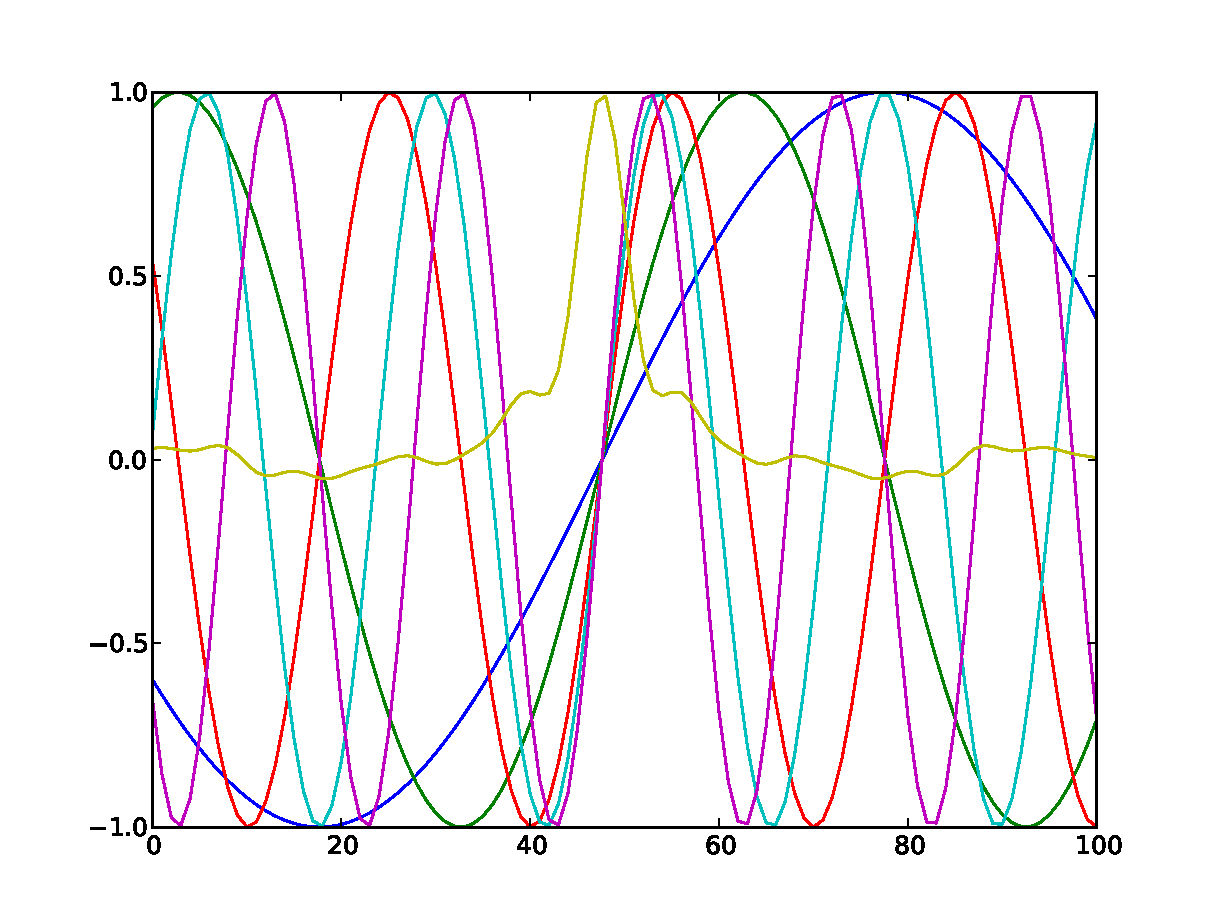
\includegraphics[width=1\textwidth]{./Figures/amplitude_phase.pdf}\caption{averages sine 
functions vs. sinc function}\label{fig:amplitude_phase}
\end{minipage}
%   \hspace{1cm} 
% \begin{minipage}{0.38\linewidth}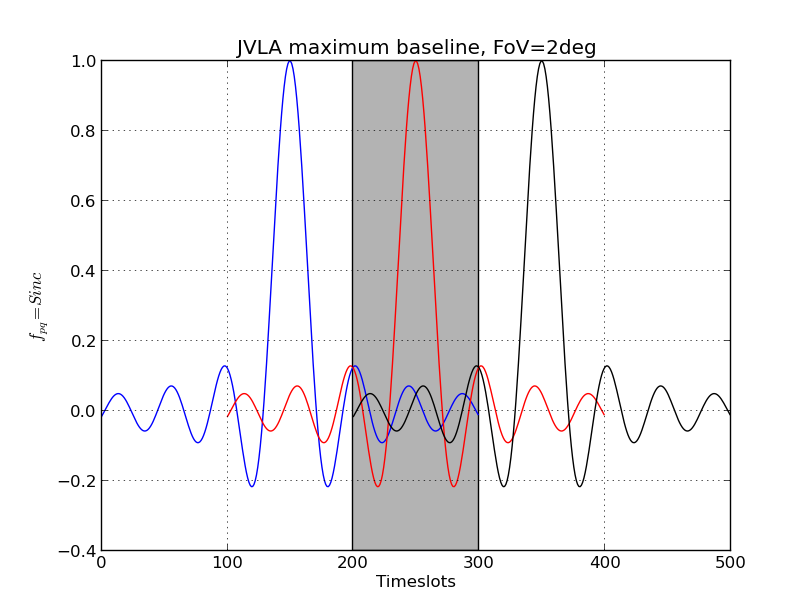
\includegraphics[width=1\textwidth]{./Figures/corrSigVLAMxBl_overlapGdelta.pdf}\caption{Overlap 
% baseline dependent windowing functions}\label{fig:corrSigVLAMxBl_overlapGdelta}\end{minipage}
\end{figure*}
\section{Simulation and comparison}
\section{Discussion and conclusion}

 \begin{acknowledgements}
 The research  made use of  MeqTrees software system designed to implement numerical models for third-generation calibration (3GC) 
 Python Extensions for Interferometry and Python. The research has been supported by the South Africa National Research Foundation.
 \end{acknowledgements}

%\bibliographystyle{aa}
%\bibliography{references}
\bibliographystyle{mn2e}
\bibliography{paper}
%\pagebreak
%\newpage
\appendix % Cue to tell LaTeX that the following 'chapters' are Appendices
% Appendix A

\section{The Fourier Transform of a top-hat windowing function} %Main appendix title
\label{AppendixA} % For referencing this appendix elsewhere, use \ref{AppendixA}
%\lhead{Appendix A. \emph{The sampled function}} % This is for the header on each page - perhaps a shortened title
A two dimensional top-hat window is defined as
\begin{alignat}{2}
\mathbf{\Pi}(\mathbf{b}) = \left\{
\begin{array}{rl}
1 & \mbox{for $\mathit{ t \times \nu \in  [t_s, t_e]\times [\nu_s, \nu_e]}$}, \\
0 & \mbox{for $\mathit{ t \times \nu  \notin [t_s, t_e]\times [\nu_s, \nu_e]}$ }
\end{array}\right.
\end{alignat}
where $[t_s, t_e]\times [\nu_s, \nu_e]$ is the passband region.
 
\begin{alignat*}{2}
\widetilde{\Pi}(\mathbf{b})&= \frac{1}{\Delta t \Delta \nu}\int_{t_s}^{t_e}\int_{\nu_s}^{\nu_e} e^{-2\pi i t\nu}dtd\nu
\end{alignat*}
Let suppose that 



%\input{Appendices/AppendixB}
%\input{Appendices/AppendixC}

%% \begin{appendix}
%% \input{Initialisation.tex}
%% \input{NoiseProps.tex}
%% \end{appendix}

\end{document}



